\section{Zielsetzung}
Im vorliegenden Experiment wird das Stefan-Boltzmann Gesetz anhand vier verschiedener Oberflächen untersucht.
Hierzu soll die Strahlungsintensität in Abhängigkeit der Temperatur sowie des Abstandes betrachtet werden.

\section{Theorie}
\label{sec:Theorie}
In der Physik ist ein Schwarzer Körper ein theoretisches Objekt, welches seine gesamte aufgenommene Strahlung vollständig in Wärmestrahlung umwandelt.
Max Planck hat für diesen Körper das Planck'sche Strahlungsgesetz entwickelt, welches sein Emissionsspektrum beschreibt.
Exemplarisch können der Grafik 1 die Spektren für einen schwarzen Körper bei verschiedenen Temperaturen entnommen werden.
\begin{figure}[H]
  \centering
  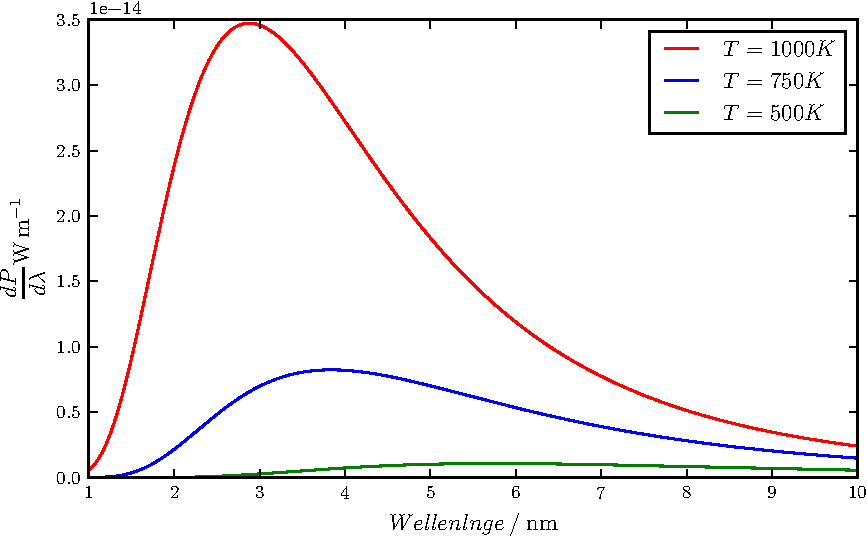
\includegraphics{plot3.pdf}
  \caption{Plot.}
  \label{fig:plot}
\end{figure}
Man kann im Allgemeinen bebobachten, dass sich das Strahlungsmaximum mit steigender Temperatur zu einer kleineren Wellenlänge und somit zu einer höheren Energie verschiebt.
Dieser Zusammenhang wird auch durch das Wiensche Verschiebungsgesetz beschrieben.\\
Zudem nimmt die gesamte Leistung, die vom schwarzen Körper abgestrahlt wird, mit ansteigender Temperatur deutlich zu.
Diese Tatsache, dass die abgestrahlte Leistung eines schwarzen Körpers von der Temperatur, und eben nur von dieser abhängt, wird durch das allgemeine Stefan-Boltzmann-Gesetz beschrieben:
\begin{equation}
  P(T) = \sigma \cdot \ T^4
\end{equation}
Hierbei bezeichnet $P$ die integrale Strahlungsdichte bezogen auf die abgestrahlte Fläche und $\sigma$ die Stefan-Boltzmann-Konstante mit dem Wert $\sigma = \SI{5.67e-8}{\watt\per\metre\tothe{2}\per\kelvin\tothe{4}}$.
Um die Strahlungseigenschaften von realen, nicht-schwarzen Körpern charakterisieren zu können, existieren verschiedene Messgrößen.\\
Das Absorptionsvermögen $A$ gibt an, welcher Anteil der auftreffenden Strahlung vom Material absorbiert wird.
Da der Körper die absorbierte Strahlung wieder als Wärme abgibt, ist das Emissionsvermögen $\epsilon$ gleich dem Absorptionsvermögen $A$.
Als dritte Materialeigenschaft existiert das Reflexionsvermögen $R$, welches angibt, welcher Anteil der Strahlung nicht absorbiert sondern reflektiert wird.
Nach dem Kirchhoffschen Strahlungsgesetz gilt der Zusammenhang
\begin{equation}
  \epsilon = 1-R.
\end{equation}
Mit diesen Messgrößen erhält der schwarze Körper das Emissionsvermögen $\epsilon = 1$, jeder reale Körper, in der Physik analog "grauer Körper" genannt, besitzt ein Emissionsvermögen von $\epsilon < 1$.
Für das Stefan-Boltzmann-Gesetz folgt mit dieser Definition für reale Körper
\begin{equation}
  P(T) = \epsilon \cdot \sigma \cdot \ T^4.
\end{equation}

\cite{sample}
